% Human Consciousness Can Construct the Universe
% Compile with: pdflatex (standard TeX Live distribution)
\documentclass[10pt,a4paper]{article}

\usepackage[utf8]{inputenc}
\usepackage[T1]{fontenc}
\usepackage{geometry}
\geometry{margin=2.5cm}

\usepackage{amsmath,amsfonts,amssymb}
\usepackage{graphicx}
\usepackage{tikz}
\usetikzlibrary{arrows.meta,positioning,calc}
\usepackage{booktabs}
\usepackage{cite}
\usepackage{hyperref}
\usepackage{algorithm,algpseudocode}

\usepackage{tabularx}
\usepackage{booktabs}
\usepackage{array}



\title{\textbf{Human Consciousness Can Construct the Universe:\\
A Chiral Coarse-Quantum Framework and Testable Predictions}}
\author{
Xiaohui Li\\
\textit{Independent Researcher, Baoji, China}\\
Correspondence: \href{mailto:danceluck@163.com}{danceluck@163.com}\\
ORCID: 0009-0003-8233-7191\\
Data homepage: \url{https://github.com/xiaohui-li-lab/}
}
\date{}

\begin{document}
\maketitle

\begin{abstract}
We propose a conceptual framework in which consciousness is treated not merely as an emergent property of the brain, but as a trans-cosmic symmetry-breaking field. This field imprints a minute chiral bias on the pre-Big-Bang quantum vacuum, which is then amplified by a self-reinforcing attraction among identical chiral modes into a universe-scale left-handedness. Human language is modeled as a coarse-grained quantum system carrying the same left-handed signature, thereby enabling the representation of microscopic quanta and the macroscopic cosmos. We formalize the conjecture, derive four testable predictions, and outline datasets, simulations, and benchmarks by which the hypothesis can be empirically confronted. The article is intentionally exploratory: it does not claim proof, but maps a route from the philosophy of mind to observational cosmology and computational linguistics.
\end{abstract}

\noindent\textbf{Keywords:} consciousness; chirality; quantum cosmology; language; homochirality; coarse-quantum framework; testable predictions

\section*{Introduction}
Human language describes electrons, galaxies, genes, and black holes. Why should a biological symbolic system be able to represent reality across more than twenty orders of magnitude? We suggest that this capacity is not accidental: language and the physical universe may share a deep structural invariant---chirality. Building on two earlier conceptual studies~\cite{Li2026a,Li2026b}, we construct a ``chiral coarse-quantum'' framework in which (i) consciousness acts from outside spacetime, (ii) it seeds a chiral asymmetry in the quantum vacuum, (iii) the resulting cosmos is left-handed, and (iv) language inherits this left-handedness at a coarse-grained level.

It must be emphasized that this is not yet an empirical claim, but a falsifiable scientific hypothesis. It reorganizes several open puzzles: the origin of cosmic homochirality~\cite{Bada1995}, parity violation in weak interactions~\cite{LeeYang1956,Wu1957}, and the ability of symbolic systems to track physical structure~\cite{UD}. Ancient narratives often place consciousness or a primordial mind prior to matter; we treat them here as cultural metaphors rather than evidence.

\section*{Theoretical Framework: The Chiral Coarse-Quantum Framework}
\subsection*{Postulates}

\noindent\textbf{Postulate 1 (Consciousness field).} Let $\mathcal{C}$ be an operator acting on a pre-geometric Hilbert space $\mathcal{H}_0$. It supplies a small chiral perturbation:
\begin{equation}
\mathcal{C}|\Psi_0\rangle = |L\rangle + \varepsilon |R\rangle,\qquad |\varepsilon|\ll 1.
\label{eq:perturbation}
\end{equation}

\noindent\textbf{Postulate 2 (Chiral amplification).} Define the chiral order parameter
\begin{equation}
\sigma = \frac{N_L - N_R}{N_L + N_R}.
\label{eq:orderparam}
\end{equation}
Identical chiral modes interact through an attractive potential
\begin{equation}
V(\chi_i,\chi_j) = -J\,\delta_{\chi_i\chi_j},\qquad J>0.
\label{eq:potential}
\end{equation}
For an initially left-biased state, the dynamics drives $\sigma\to +1$, producing a homochiral universe.

\noindent\textbf{Postulate 3 (Language as a chiral mirror).} A linguistic representation $\mathcal{L}$ is a coarse-grained quantum state $|\psi_L\rangle$ in $\mathcal{H}_L$. It maps to a physical state $|\psi_U\rangle$ via a chirality-preserving isometry $\Phi:\mathcal{H}_L\to\mathcal{H}_U$:
\begin{equation}
\langle\psi_L|\chi_L|\psi_L\rangle = \langle\psi_U|\chi_U|\psi_U\rangle.
\label{eq:language}
\end{equation}

This formalization corresponds to the ``grandfather--father--grandson'' intuition: consciousness generates the universe, the universe generates embodied language, and consciousness also acts directly on language.

\begin{figure}[htbp]
\centering
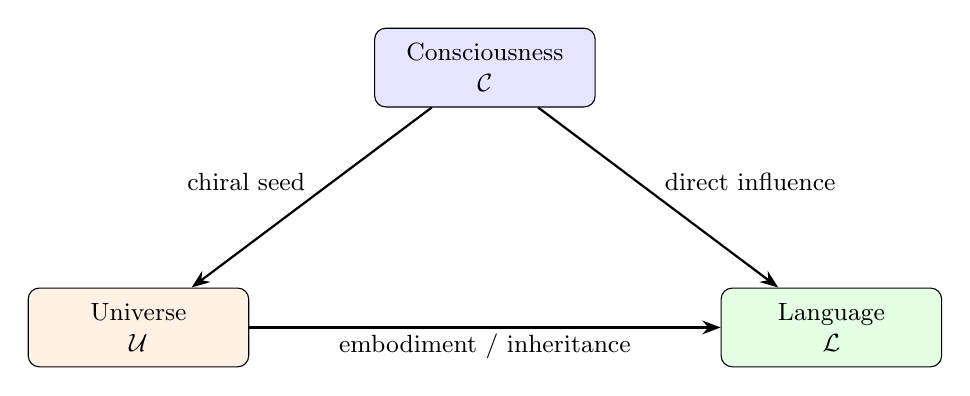
\begin{tikzpicture}[
  scale=1.1,
  every node/.style={font=\small},
  box/.style={draw, rounded corners, minimum width=2.8cm, minimum height=1cm, align=center}
]
\node[box, fill=blue!10] (C) at (0,3) {Consciousness\\$\mathcal{C}$};
\node[box, fill=orange!10] (U) at (-4,0) {Universe\\$\mathcal{U}$};
\node[box, fill=green!10] (L) at (4,0) {Language\\$\mathcal{L}$};

\draw[-{Stealth}, thick] (C) -- (U) node[midway, above left, fill=white, inner sep=2pt] {chiral seed};
\draw[-{Stealth}, thick] (C) -- (L) node[midway, above right, fill=white, inner sep=2pt] {direct influence};
\draw[-{Stealth}, thick] (U) -- (L) node[midway, below, fill=white, inner sep=2pt] {embodiment / inheritance};
\end{tikzpicture}
\caption{Causal hierarchy: consciousness (grandfather) acts both on the universe (father) and directly on language (grandson); the universe also influences language through embodiment.}
\label{fig:hierarchy}
\end{figure}

\subsection*{Cosmic chiral amplification mechanism}
In the hypothetical Pre-Big-Bang phase, the vacuum is chirally degenerate. The perturbation $\varepsilon$ from the consciousness field $\mathcal{C}$ lifts the degeneracy so that the occupation number of left-handed modes $N_L$ slightly exceeds $N_R$. By Eq.~\eqref{eq:potential}, same-chiral modes attract and opposite-chiral modes repel, leading to exponential symmetry breaking. The process can be approximated by a Gross--Pitaevskii-type or Ising-like spin model. The critical condition for the phase transition is
\begin{equation}
h > h_c(T),
\end{equation}
where $h$ is the effective chiral strength of the consciousness field and $T$ is a pre-geometric ``temperature.'' When $T<T_c$ and $h$ exceeds the threshold, the system spontaneously enters a homochiral phase with $\sigma\approx +1$.

\begin{figure}[htbp]
\centering
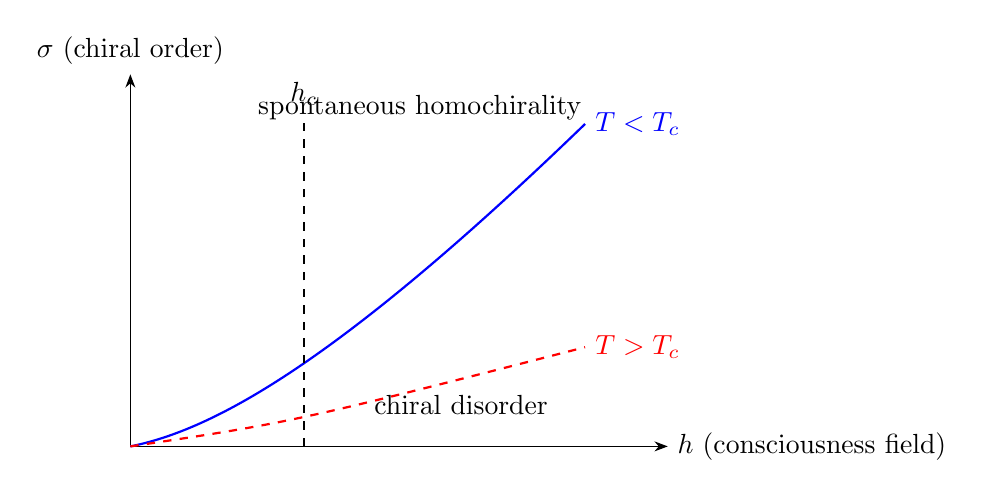
\begin{tikzpicture}[scale=1.05]
\draw[-{Stealth}] (0,0) -- (6.5,0) node[right] {$h$ (consciousness field)};
\draw[-{Stealth}] (0,0) -- (0,4.5) node[above] {$\sigma$ (chiral order)};
\draw[thick, blue] (0,0) .. controls (1,0.2) and (2.5,1.0) .. (5.5,3.9) node[right] {$T<T_c$};
\draw[thick, dashed, red] (0,0) .. controls (2,0.3) .. (5.5,1.2) node[right] {$T>T_c$};
\draw[dashed] (2.1,0) -- (2.1,4) node[above] {$h_c$};
\node at (3.5,4.1) {spontaneous homochirality};
\node at (4,0.5) {chiral disorder};
\end{tikzpicture}
\caption{Phase diagram of chiral order parameter $\sigma$ versus consciousness field $h$: for $T<T_c$, the system spontaneously enters a left-handed homochiral phase once $h$ exceeds the critical value $h_c$.}
\label{fig:phase}
\end{figure}

\subsection*{Language as a chiral carrier}
Language is not consciousness itself, but its embodied expression. Because linguistic systems evolve under the influence of the same source-consciousness, their syntactic-semantic structures are hypothesized to carry the same left-handed signature as the cosmos. Specifically, the helicity of dependency syntax trees, the directionality of semantic composition, and the recursive architecture of symbol generation can all be quantified by a signed ``linguistic chirality index'' $\tau$. A significantly positive $\tau$ would support the hypothesis that language and the universe share left-handedness.

\section*{Testable Predictions}

\begin{enumerate}
\item \textbf{Cosmic large-scale chirality.} CMB temperature and polarization maps, together with galaxy spin catalogs, will show a statistically significant left-handed helicity on scales $\gtrsim 1$~Gpc, exceeding the standard statistically isotropic model at $\ge 3\sigma$ confidence.
\item \textbf{Weak-interaction baseline.} Neutrinos will remain left-handed within experimental precision; any right-handed neutrino component in the early universe must be below $10^{-10}$.
\item \textbf{Linguistic chirality.} Across at least 50 unrelated languages, dependency syntax trees will exhibit a universal left-handed helical bias, measured by a signed tree-chirality index $\tau>0$ with $p<0.001$ against a random-tree null model.
\item \textbf{Laboratory chiral condensate.} Under parity-violating electroweak forces, a cold chiral molecular condensate will undergo a phase transition to a homochiral ground state at a predicted critical field $B_c$, whose order of magnitude is approximately $10^{-7}$--$10^{-6}$~T (to be refined with specific molecular magnetic moments).
\end{enumerate}

\section*{Methods, Validation, and Benchmarks}
\subsection*{Cosmological chirality estimator}
Using Planck 2018 CMB data~\cite{Planck2018VI} and forthcoming Simons Observatory / CMB-S4 data, we construct a new chirality statistic
\begin{equation}
S_\ell = \frac{\langle (a_{\ell m}^E)^* a_{\ell m}^B\rangle_m}{\sigma_\ell},
\end{equation}
where $E$ and $B$ denote electric-type and magnetic-type polarization modes. The measured $S_\ell$ is compared with $10^3$ Monte Carlo isotropic simulations to compute the false-positive rate, and cross-checked with LSST~\cite{LSST2009} and DESI~\cite{DESI2016} galaxy spin maps.

\subsection*{Particle-physics constraints}
Atmospheric neutrino data from IceCube and effective neutrino-mass measurements from KATRIN are used to constrain the right-handed neutrino mixing angle. A right-handed component below $10^{-10}$ would be consistent with the framework.

\subsection*{Linguistic chirality}
Parse the Universal Dependencies corpora~\cite{UD}; for each language build dependency syntax trees and compute the signed tree-chirality index $\tau$. Use 10-fold cross-language validation and permutation tests to control for cultural borrowing and genealogical relatedness.

\subsection*{Spin-network simulation and benchmark}
We propose Algorithm~\ref{alg:spin}.

\begin{algorithm}[htbp]
\caption{Chiral spin-network Monte Carlo}\label{alg:spin}
\begin{algorithmic}[1]
\State Initialize $N=10^4$ spins $\chi_i\in\{L,R\}$ with a small left bias.
\State Set $J/kT=1.2$, $h=10^{-3}$.
\For{sweep $=1$ to $10^6$}
  \For{each node $i$}
    \State Propose a flip $\chi_i\to -\chi_i$.
    \State Accept with probability $\min\{1,\exp(-\Delta E/kT)\}$.
  \EndFor
  \If{sweep mod 100 $=0$}
    \State Measure $\sigma$ and Binder cumulant $U_L$.
  \EndIf
\EndFor
\State Compare $\sigma(h)$ and critical exponents with 2D Ising benchmark.
\end{algorithmic}
\end{algorithm}

The benchmark is the exact solution of the two-dimensional Ising model, for which $\beta_c=\ln(1+\sqrt{2})/2$. If the critical behavior in the $h\to 0$ limit agrees with the Ising universality class, the algorithm is validated. Example parameters are given in Table~\ref{tab:params}.


\begin{table}[htbp] \centering \caption{Proposed observations, experiments, and validation schemes.} \begin{tabularx}{\textwidth}{@{}>{\raggedright\arraybackslash}p{2cm}X>{\raggedright\arraybackslash}p{3.2cm}>{\raggedright\arraybackslash}p{3.2cm}@{}}  \toprule \textbf{Domain} & \textbf{Data / Experiment} & \textbf{Expected signal} & \textbf{Validation} \\ \midrule Cosmology & Planck/SO/CMB-S4 CMB; LSST/DESI galaxy spins & Large-scale left-handed helicity $\ge3\sigma$ & Isotropic Monte Carlo simulations \\ Particle physics & IceCube/KATRIN neutrinos & Right-handed component $<10^{-10}$ & Bayesian parameter estimation \\ Linguistics & Universal Dependencies, $\ge$50 languages & Dependency-tree $\tau>0$, $p<0.001$ & Permutation test, cross-language validation \\ Laboratory & Cold chiral molecular condensate & Homochiral transition at predicted $B_c$ & Scaling analysis at transition point \\ \bottomrule \end{tabularx} \label{tab:obs} \end{table}





\begin{table}[htbp]
\centering
\caption{Example parameters for the spin-network simulation.}
\begin{tabular}{@{}lll@{}}
\toprule
\textbf{Parameter} & \textbf{Value} & \textbf{Description} \\ \midrule
$N$ & $10^4$ & Number of lattice nodes \\
$J/kT$ & $1.2$ & Same-chirality coupling strength \\
$h$ & $10^{-3}$ & Effective chiral external field \\
Sweeps & $10^6$ & Number of Metropolis updates \\
Sampling interval & 100 steps & Thinning for autocorrelation \\
Benchmark & Exact 2D Ising solution & $\beta_c=\ln(1+\sqrt{2})/2$ \\ \bottomrule
\end{tabular}
\label{tab:params}
\end{table}

\section*{Discussion}
This framework places consciousness, cosmos, and language into a unified causal hierarchy: consciousness, existing beyond the universe, shapes the universe through a chiral seed and also acts directly on embodied language. This view is not equivalent to the multiverse hypothesis; it is a new cosmology and a new theory of consciousness that takes consciousness as first principles. Nevertheless, it remains highly speculative. Its scientific value depends on whether future observations in CMB, neutrino physics, biological homochirality, and linguistic structure reveal consistent and reproducible left-handed signals.

\section*{Author Contributions}
Xiaohui Li conceived the framework, wrote the manuscript, designed the proposed experiments and simulations, and prepared the conceptual figures.

\section*{Data Availability}
Cosmological data are public: Planck, SDSS, and LSST (upon release). Linguistic corpora are from Universal Dependencies~\cite{UD}. Simulation inputs and outputs will be deposited at \url{https://github.com/xiaohui-li-lab/2026-11-9/}.

\section*{Code Availability}
Python/C++ scripts for spin-network simulation, CMB chirality estimator, and linguistic chirality index will be deposited at the same GitHub repository.

\section*{Competing Interests}
The author declares no competing interests.

\begin{thebibliography}{99}
\bibitem{Li2026a}
X. Li, ``What is consciousness, and its eleven explanations: eleven theses on the nature, attachment, and transcendence of consciousness,'' manuscript in preparation (2026).

\bibitem{Li2026b}
X. Li, ``Human language as the reason for describing microscopic quanta and the macroscopic cosmos: a chiral coarse-quantum framework,'' manuscript in preparation (2026).

\bibitem{Planck2018VI}
Planck Collaboration, ``Planck 2018 results. VI. Cosmological parameters,'' \textit{Astronomy \& Astrophysics} \textbf{641}, A6 (2020).

\bibitem{Planck2018X}
Planck Collaboration, ``Planck 2018 results. X. Constraints on inflation,'' \textit{Astronomy \& Astrophysics} \textbf{641}, A10 (2020).

\bibitem{LeeYang1956}
T. D. Lee and C. N. Yang, ``Question of Parity Conservation in Weak Interactions,'' \textit{Physical Review} \textbf{104}, 254 (1956).

\bibitem{Wu1957}
C. S. Wu, E. Ambler, R. W. Hayward, D. D. Hoppes, and R. P. Hudson, ``Experimental Test of Parity Conservation in Beta Decay,'' \textit{Physical Review} \textbf{105}, 1413 (1957).

\bibitem{Bada1995}
J. L. Bada, ``Origins of homochirality,'' \textit{Nature} \textbf{374}, 594 (1995).

\bibitem{UD}
Universal Dependencies, \url{https://universaldependencies.org/}.

\bibitem{LSST2009}
LSST Science Collaboration, ``LSST Science Book,'' arXiv:0912.0201 (2009).

\bibitem{DESI2016}
DESI Collaboration, ``The DESI Experiment Part I: Science, Targeting, and Survey Design,'' arXiv:1611.00036 (2016).

\bibitem{LiddleLyth2000}
A. R. Liddle and D. H. Lyth, \textit{Cosmological Inflation and Large-Scale Structure} (Cambridge University Press, 2000).

\bibitem{Coleman1977}
S. R. Coleman, ``Fate of the false vacuum: Semiclassical theory,'' \textit{Physical Review D} \textbf{15}, 2929 (1977).
\end{thebibliography}

\end{document}
